\chapter{Teorie}
\newacronym{er}{ER}{Entity-Relationship}

V~této kapitole představíme potřebné teoretické koncepty, kterých bude využívat výsledná aplikace.
Mezi tyto koncepty patří \acrfull{er}, schematická kategorie včetně teorie kategorií a vizuální diagram schematické kategorie.

\section{Entity Relationship}

Datový model \acrfull{er} poprvé představil Chen už v~roce 1976~\cite{chen_entity-relationship_1976}.
Od té doby se však \acrshort{er} vyvíjel, jak se potřeby datového modelování rozšiřovaly.
\acrshort{er} není standardizováno, ale jednu moderní verzi představili Atzeni, Ceri, Paraboschi a Torlone~\cite[s.~163-179]{atzeni_database_1999}.
Na jejich \acrshort{er} modelu založíme ten náš, který zde popíšeme.

V~tabulce~\ref{tab:er-constructs} jsou vyobrazeny jednotlivé konstrukty \acrshort{er} modelu.
Zde blíže popíšeme sémantiku jednotlivých konstruktů:
\begin{itemize}
  \item Entitní typ (Entity Type) reprezentuje entitu.
        Každá entita má jméno.
  \item Vztahový typ (Relationship Type) reprezentuje vztah mezi dvěma a více (ne nutně různými) entitami.
        Každý vztah má jméno.
  \item Atribut (Attribute) reprezentuje atribut/vlastnost entitních nebo vztahových typů.
        Každý atribut má jméno.
  \item Složený atribut (Composite Attribute) je atribut, který má sám atributy.
        Zakazujeme však další větvení, tedy atributy složeného atributu už samy nemohou být složené.
        Každý složený atribut má sám jméno, podobně jako jeho vlastní atributy.
  \item \label{def:cardinality}Kardinalita (Cardinality) je dvojice $(a, b) \in \set{\zero, \one}\times \set{\one, \many}$, kde $a$ nazýváme minimální kardinalita (spodní hranice) a $b$ maximální kardinalita (horní hranice).
        Kardinalitu musí mít všechny atributy a každý účastník vztahu.
        Výchozí kardinalita je $(1, 1)$ a ve schématu se většinou neuvádí.
        Spodní hranice 0 znamená, že účast je volitelná; hranice 1 znamená, že účast je povinná.
        Horní hranice 1 znamená, že účast je nejvýše jedna; hranice~\many{} znamená, že účastí je libovolný počet.
        \begin{itemize}
          \item Hranice kardinalit pro jednotlivé účastníky vztahů vyjadřují minimální a resp. maximální počet výskytů jednotlivých instancí účastníků v~tomto vztahu.
          \item Hranice kardinalit u~atributů vyjadřují minimální a resp. maximální počet hodnot atributu, které se vztahují ke každé instanci entity/vztahu.
        \end{itemize}
  \item Identifikátor (Identifier) umožňuje jednoznačně rozlišit (identifikovat) instance entit.
        Pro každý entitní typ je povinný alespoň jeden identifikátor, ale může jich být více.
        Každý identifikátor je tvořen buď
        \begin{itemize}
          \item jedním nebo více atributy daného entitního typu; takový identifikátor nazýváme interní, nebo
          \item jedním, nebo více vztahovými typy, jehož se daná entita účastní, případně kombinací s~předchozím; takový identifikátor nazýváme externí.
        \end{itemize}
  \item Zobecnění (generalization), nebo také ISA hierarchie\footnote{ISA z anglického \enquote{is a}, analogicky ke vztahu \enquote{has a}} (ISA hierarchy), vyjadřuje vztah podobný dědičnosti v objektově orientovaném programování.
        Jde o vztah mezi entiním typem $E$ zvaným \emph{rodič} a jedním nebo více \emph{dětmi} $E_1, \dots, E_n$.
        Všechny vlastnosti rodiče (atributy, identifikátory, spojené vztahové typy a další ISA hierarchie) jsou i vlastnosti každého z dětí.
        Každý výskyt dítěte je také výskytem rodiče.
\end{itemize}

Entitní typy, které nemají ani jeden interní identifikátor (musí mít tedy externí), nazýváme \emph{slabé} entitní typy (weak entity types).
Pokud mají interní identifikátor, nazýváme je \emph{silné} entitní typy (strong entity types).

Jednoho vztahu se může účastnit nejvýše jeden slabý entitní typ, protože pro dva takové by byla identifikace nesmyslná.
Externí identifikace se však může řetězit, jako na obrázku~\ref{fig:er-external-identifier-chain}.
Nesmí ovšem vzniknout cyklus a to ani v kombinaci s ISA hierarchiemi.
Formálněji -- pokud vytvoříme orientovaný graf $G=(V,E)$ takový, že
\begin{itemize}
  \item $V = \textit{entitní typy }\cup\textit{vztahové typy}$ a
  \item do hran $E$ přidáme
        \begin{itemize}
          \item pro externí identifikátory všechny hrany na orientované cestě od identifikovaného k identifikujícímu entitnímu typu,
          \item pro ISA hierarchii pro každý vztah rodič-dítě, kde $a$ je dítě a $b$ je rodič, hranu $(a, b)$,
        \end{itemize}
\end{itemize}
pak graf $G$ musí být acyklický.

Slabý entitní typ musí být v daném vztahu s kardinalitou $(\one,\one)$.
To proto, že když je instance entity identifikována vztahem, musí tento vztah být jednoznačný -- právě jeden.

\begin{figure}[!htb]
  \centering
  \missingfigure{\Huge Zřetězení externích identifikátorů}
  \caption{Zřetězení externích identifikátorů}
  \label{fig:er-external-identifier-chain}
\end{figure}

Atributy v~\acrshort{er} by měly být pouze elementární vlastnosti.
Například pokud by měla mít entita \enquote{Zákazník} atribut \enquote{Fyzická adresa}, může být vhodnější fyzickou adresu modelovat jako entitu, neboť má sama atributy jako \enquote{Ulice} a \enquote{Město}.
Pokud ale víme, že jiná entita nebude v~modelu mít fyzickou adresu, můžeme ji případně modelovat jako složený atribut.

U~kardinality poznamenáme, že se v~\acrshort{er} modelu často dovoluje použít jako hranice libovolná nezáporná celá čísla, tedy $(a, b)\in \mathbb N_0\times \left(\mathbb N_0 \cup \set{\many}\right)$, tž.~$a\leq b$ (dodefinujeme $\forall a\colon a < \many$).
Dají se tak vyjádřit přesnější omezení, např. že jeden uživatel může mít maximálně 5 bankovních účtů.
Ve většině případů ale stačí námi definované hranice kardinality, které vyjadřují volitelnost/povinnost pro spodní hranici a jednočetnost/mnohočetnost pro horní hranici.
Toto vymezení nám umožní vyjádřit čtyři nejdůležitější případy, nad kterými se při modelování uvažuje.

Dále upozorníme, že místo~\many{} se v~\acrshort{er} modelu může použít symbol \texttt{n} nebo \texttt{N} pro vyjádření \enquote{libovolného počtu}.
Důležitá je ale konzistentnost, aby se v~jednom modelu nevyskytovaly dva různé symboly, což by mohlo zmást čtenáře.
V~této práci budeme používat pouze symbol~\many{}.

\begin{table}[!htb]
  \centering
  \begin{tabular}{@{}rm{7cm}@{}} \toprule
    Konstrukt             & Grafická reprezentace                                     \\ \midrule
    Entitní typ           & {\centering
\includegraphics{../img/er-model/entity.pdf}}  \\
    Vztahový typ          & 
\includegraphics{../img/er-model/relationship.pdf}        \\
    Atribut               & 
\includegraphics{../img/er-model/attribute.pdf}           \\
    Složený atribut       & 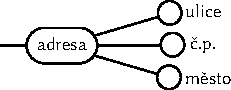
\includegraphics{../img/er-model/composite-attribute.pdf} \\
    Interní identifikátor & 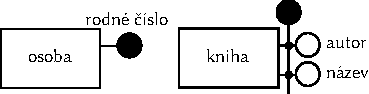
\includegraphics{../img/er-model/identifier.pdf}          \\
    Externí identifikátor & 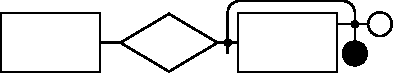
\includegraphics{../img/er-model/external-identifier.pdf} \\
    Zobecnění             & 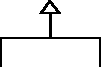
\includegraphics{../img/er-model/generalization.pdf}      \\ \bottomrule
  \end{tabular}
  \caption[Grafická reprezentace konstruktů \acrshort{er} modelu]{Grafická reprezentace konstruktů \acrshort{er} modelu, upraveno a přeloženo~\cite[s.~164]{atzeni_database_1999}}
  \label{tab:er-constructs}
\end{table}

\section{Schematická kategorie}

Nejdříve popíšeme kategorii z~teorie kategorií, na níž je schematická kategorie založena.

Kategorie je matematická struktura, která zobecňuje ostatní struktury.
Umožňuje mimo jiné studovat vztahy mezi nimi.
Poprvé byla představena Eilenbergem a MacLanem v~roce 1945~\cite{eilenberg_1945}.

Kategorie $C=(\mathcal O, \mathcal M, \circ)$ se skládá
z~\begin{itemize}
  \item třídy objektů $\mathcal O$,
  \item třídy morfismů $\mathcal M$; každý morfismus $f \in \mathcal M$ má zdrojový objekt $A\in\mathcal O$, cílový objekt $B\in\mathcal O$ a říkáme $f: A\to B$ ($f$ je morfismus z~$A$ do $B$),
  \item operace skládání $\circ\colon \mathcal M\times\mathcal M \to \mathcal M$; pro každé dva morfismy $f\colon A\to B, g\colon B\to C$ musí $g\circ f\in \mathcal M$ (tranzitivita); pro tuto operaci navíc platí axiomy:
        \begin{itemize}
          \item asociativita -- pro morfismy $f\colon A\to B, g\colon B\to C, h\colon C\to D$ platí $h\circ (g \circ f) = (h\circ g)\circ f$,
          \item identita -- pro každý objekt $A$ existuje identita $1_A$, tž. $f\circ 1_A = f = 1_B\circ f$ pro každý morfismus $f: A\to B$.
        \end{itemize}
\end{itemize}

Kategorie je často vizuálně reprezentována schématem připomínajícím orientovaný graf, kde vrcholy jsou objekty a hrany morfismy.
Příklad této vizualizace je na obrázku~\ref{fig:category-example-all}.
Jedná se o~kategorii se čtyřmi objekty $A, B, C, D$.
V~této práci vizualizaci kvůli schematické kategorii budeme zjednodušovat tak, že v~ní vynecháme určité morfismy, které budeme považovat za implicitní.
Těmito morfismy jsou takové, které jsou v~kategorii jen kvůli tranzitivitě, a takové, které jsou v~kategorii jen kvůli splnění axiomu identity.
Někdy budou tyto morfismy důležité, v~takovém případě je v~obrázku explicitně uvedeme.
Zjednodušená vizualizace je na obrázku~\ref{fig:category-example-no-deduced}.
Všimněme si, že identity (např. $1_A$) a složené morfismy (např. $i\circ f$) ve schématu nejsou, tedy jsou implicitní.

\begin{figure}[!htb]
  \shorthandoff{"}
  \centering
  \begin{subfigure}{.45\textwidth}
    \centering
    \begin{tikzcd}
      % https://tikzcd.yichuanshen.de/#N4Igdg9gJgpgziAXAbVABwnAlgFyxMJZABgBpiBdUkANwEMAbAVxiRAEEQBfU9TXfIRQBGclVqMWbAELdeIDNjwEiZYePrNWiEAGE5fJYKKj11TVJ0ARbuJhQA5vCKgAZgCcIAWyRkQOCCQAJnNJbRAHEGoGOgAjGAYABX5lIRB3LAcACxwDEA9vYOoApABmUK02LKiQGPiklOMdDOzcnjdPH0RRf0DEcolKnSw8gq6-Eu6Ky3zRzt9ivoGLcKyAHTWAYyx3TYACBwBePawN7d291xq6hOSjFWGwbFg5wsQJvr8GCAg0IiCAOxkVyMOAwcQ3Br3NItHI1LIwOhQJBgJgMBjTcLCAD6nHa+XmU16SB631+RAAnMDQeDonFbo0HulMnDMWwcbJ8WMyosebUfn8UFTSCCGGCIfSoQImbDcmydDibFzCSFiYhVWTBchAdSxbTapK7tKYSy5YMZjj9FwKFwgA
      A~\arrow[d, "g"'] \arrow[r, "f"] \arrow[rd, "h\circ g= i\circ f" description] \arrow["1_A"', loop, distance=2em, in=215, out=145] & B \arrow[d, "i"] \arrow["1_B"', loop, distance=2em, in=35, out=325] \\
      C \arrow[r, "h"'] \arrow["1_C"', loop, distance=2em, in=215, out=145]                                                             & D \arrow["1_D"', loop, distance=2em, in=35, out=325]
    \end{tikzcd}%
    \caption{Se všemi morfismy}%
    \label{fig:category-example-all}
  \end{subfigure}
  \begin{subfigure}{.45\textwidth}
    \centering
    \begin{tikzcd}
      A~\arrow[r, "f"] \arrow[d, "g"] & B \arrow[d, "i"] \\
      C \arrow[r, "h"]                & D
    \end{tikzcd}
    \caption{Bez tranzitivních a identitních morfismů}%
    \label{fig:category-example-no-deduced}
  \end{subfigure}%
  \caption{Příklad kategorie}%
  \label{fig:category-example}%
  \shorthandon{"}
\end{figure}

Schematická kategorie je zobecnění databázových schémat založená na teorii kategorií.
Jedná se o~kategorii, jejíž objekty odpovídají jednotlivým entitním typům, atributům a vztahovým typům \acrshort{er} schématu.
Morfismy odpovídají vztahům mezi těmito objekty, přičemž aby byly splněny axiomy kategorie, musí se přidat navíc identity a tranzitivní uzávěr těchto morfismů.
Tento koncept společně s~algoritmem převodu z~\acrshort{er} schématu do schematické kategorie uvádí Martin Svoboda, Pavel Čontoš a Irena Holubová~\cite{svoboda_categorical_2021}.
Pro naše účely se v~této práci nebudeme řídit přesně podle této originální publikace, nýbrž schematickou kategorii lehce upravíme.

Schematická kategorie se tedy skládá z~třídy objektů a třídy morfismů.

Objekt je čtveřice (identita, název, data $D$, množina identifikátorů $I$).
Identita je libovolný symbol (např. z~$\mathbb N$), který rozlišuje a unikátně identifikuje objekty, které mají ostatní složky totožné.
Název popisuje textovým řetězcem o~jaký objekt se jedná a je zde pro uživatele (čtenáře schematické kategorie).
Data je množina tzv. \emph{properties} a platí $I\subseteq \mathcal P(D)$, tedy je to nadmnožina jednotlivých properties zmíněných v~identifikátorech.
Každý identifikátor sestává z~properties a množina všech identifikátorů je pak množina sestávající z~identifikátorů daného objektu.
Každý objekt musí mít nejméně jeden identifikátor.
Musí platit $D\supseteq \bigcup I$.
Pro ilustraci -- při převodu z~\acrshort{er} bude pro původní entitní typy a atributy platit $D = \bigcup I$, ale u~vztahových typů může být v~$D$ něco navíc.

Morfismus je osmice (signatura, doména, kodoména, směr, název, kardinalita, duplicity, uspořádání).
Signatura vyjadřuje \enquote{cestu}.
Jedná se o~řetězec složený ze signatur jednotlivých morfismů, z~kterých se morfismus skládá.
Pokud se z~dalších morfismů neskládá, je signatura unikátní identitou morfismu (symbol).
Pro ilustraci viz obrázek~\ref{fig:morphism-signatures}.

Doména a kodoména jsou identity příslušných objektů, odpovídají tak zdrojovému a cílovému objektu kategorie.

Směr udává směr morfismu (který nemusí nutně odpovídat dvojici doména/kodoména).
To proto, že pro každý morfismus bude existovat jeho protějšek.
Směr má dvě možné hodnoty a budeme je značit \one{} (tam), \zero{} (zpět).

Kardinalita odpovídá tomu, jak byla popsána pro \acrshort{er} v~sekci~\ref{def:cardinality} na straně~\pageref{def:cardinality}.
Při skládání se kardinality transformují následovně: pro kardinality $(a, b)$ a $(c, d)$ je jejich složením $(\min(a, c), \max(b, d))$.
Uspořádání nad symboly kardinalit je intuitivně $\zero < \one < \many$.

Duplicity a uspořádání jsou booleovské hodnoty (\texttt{true}/\texttt{false}).
Mají význam pouze pokud je maximální kardinalita~\many.
Říkají, zda-li jsou v instanci modelu u objektů spojených daným morfismem povoleny duplicitní objekty, respektive jestli u nich záleží na pořadí.

Morfismy ve schematické kategorii rozdělíme na několik druhů, které jsou všechny vidět na obrázku~\ref{fig:morphism-signatures}:
\begin{itemize}
  \item \emph{bázové} (base) morfismy jsou ty, které odpovídají jednotlivým spojením a ISA hierarchiím mezi objekty; signatura je identita,
  \item \emph{identitní} (identity) morfismy jsou ty, které vznikly kvůli axiomu identity; signatura je $\varepsilon$,
  \item \emph{odvozené} (composite) morfismy jsou ty, které vznikly kvůli tranzitivitě; signatura je opravdová cesta (zřetězené signatury); zřetězování zapisujeme ve stejném pořadí jako skládání morfismů, aby bylo analogické.
\end{itemize}

\begin{figure}[!htb]
  \centering
  \begin{tikzpicture}
    \tikzset{vertex/.style={shape=circle,draw,minimum size=1em}}
    \tikzset{edge/.style = {->,> = latex'}}
    \node[vertex] (a) {};
    \node[vertex] (b) [right=of a] {};
    \node[vertex] (c) [right=of b] {};

    \draw[edge] (a) to[bend left] node[above] {$13$} (b) ;
    \draw[edge] (b) to[bend left] node[above] {$7$}  (c);
    \draw[edge] (a) to[bend right] node[below] {$7\cdot 13$} (c);
    \draw[edge] (a) to[loop left] node[left] {$\varepsilon$} (a);
    \draw[edge] (b) to[loop above] node[above] {$\varepsilon$} (b);
    \draw[edge] (c) to[loop right] node[right] {$\varepsilon$} (c);
  \end{tikzpicture}
  \caption{Signatury morfismů, $\cdot$ je operace konkatenace (zřetězování) symbolů}
  \label{fig:morphism-signatures}
\end{figure}

% \section{Převod \acrshort{er} na schematickou kategorii}
% 
% \begin{figure}[!htb]
%   \centering
%   \missingfigure{\Huge příklad \acrshort{er} modelu a jeho převodu na schematickou kategorii}
%   \caption{\acrshort{er} model a jeho odpovídající schematická kategorie}
%   \label{fig:test}
% \end{figure}
